%======================================================================
\chapter{Requirement Specification \& Methodology}
%======================================================================

\section{Software Development Life Cycle (SDLC)}
METRIX is developed using an \textbf{Agile and Iterative Methodology} over a four-week delivery timeline. Given the multi-stakeholder nature of legal metrology, requirements and interfaces are developed and validated in weekly sprint increments:
\begin{itemize}
    \item \textbf{Week 1 (Sprint 1):} Requirement analysis, modular monolith architecture, database schema, and JWT-based authentication with Role-Based Access Control (RBAC).
    \item \textbf{Week 2 (Sprint 2):} Instrument registration catalog, guided verification application wizard, and multi-state application tracking.
    \item \textbf{Week 3 (Sprint 3):} Inspection scheduling, digital MPE observation recording, and ReportLab PDF certificate generation with embedded QR codes.
    \item \textbf{Week 4 (Sprint 4):} Public QR verification portal, automated expiry monitoring, role-specific dashboards, and integration testing.
\end{itemize}

\section{Actor Roles and Use Case Diagram}
The system defines five primary actors:
\begin{itemize}
    \item \textbf{Instrument Owner / Business:} Registers instruments, submits verification applications, uploads payment challans, and tracks certificate status.
    \item \textbf{Legal Metrology Officer (LMO):} Reviews district applications, conducts physical inspections, records error observations, and issues digital certificates.
    \item \textbf{Government Approved Test Centre (GATC):} Receives specialized instrument verification tasks and logs official calibration observations.
    \item \textbf{Administrator:} Oversees user accounts, allocates inspection queues, and monitors district compliance dashboards.
    \item \textbf{Public / Citizen Consumer:} Scans certificate QR codes to verify calibration authenticity in real time without requiring login credentials.
\end{itemize}

\begin{figure}[htbp]
\centering
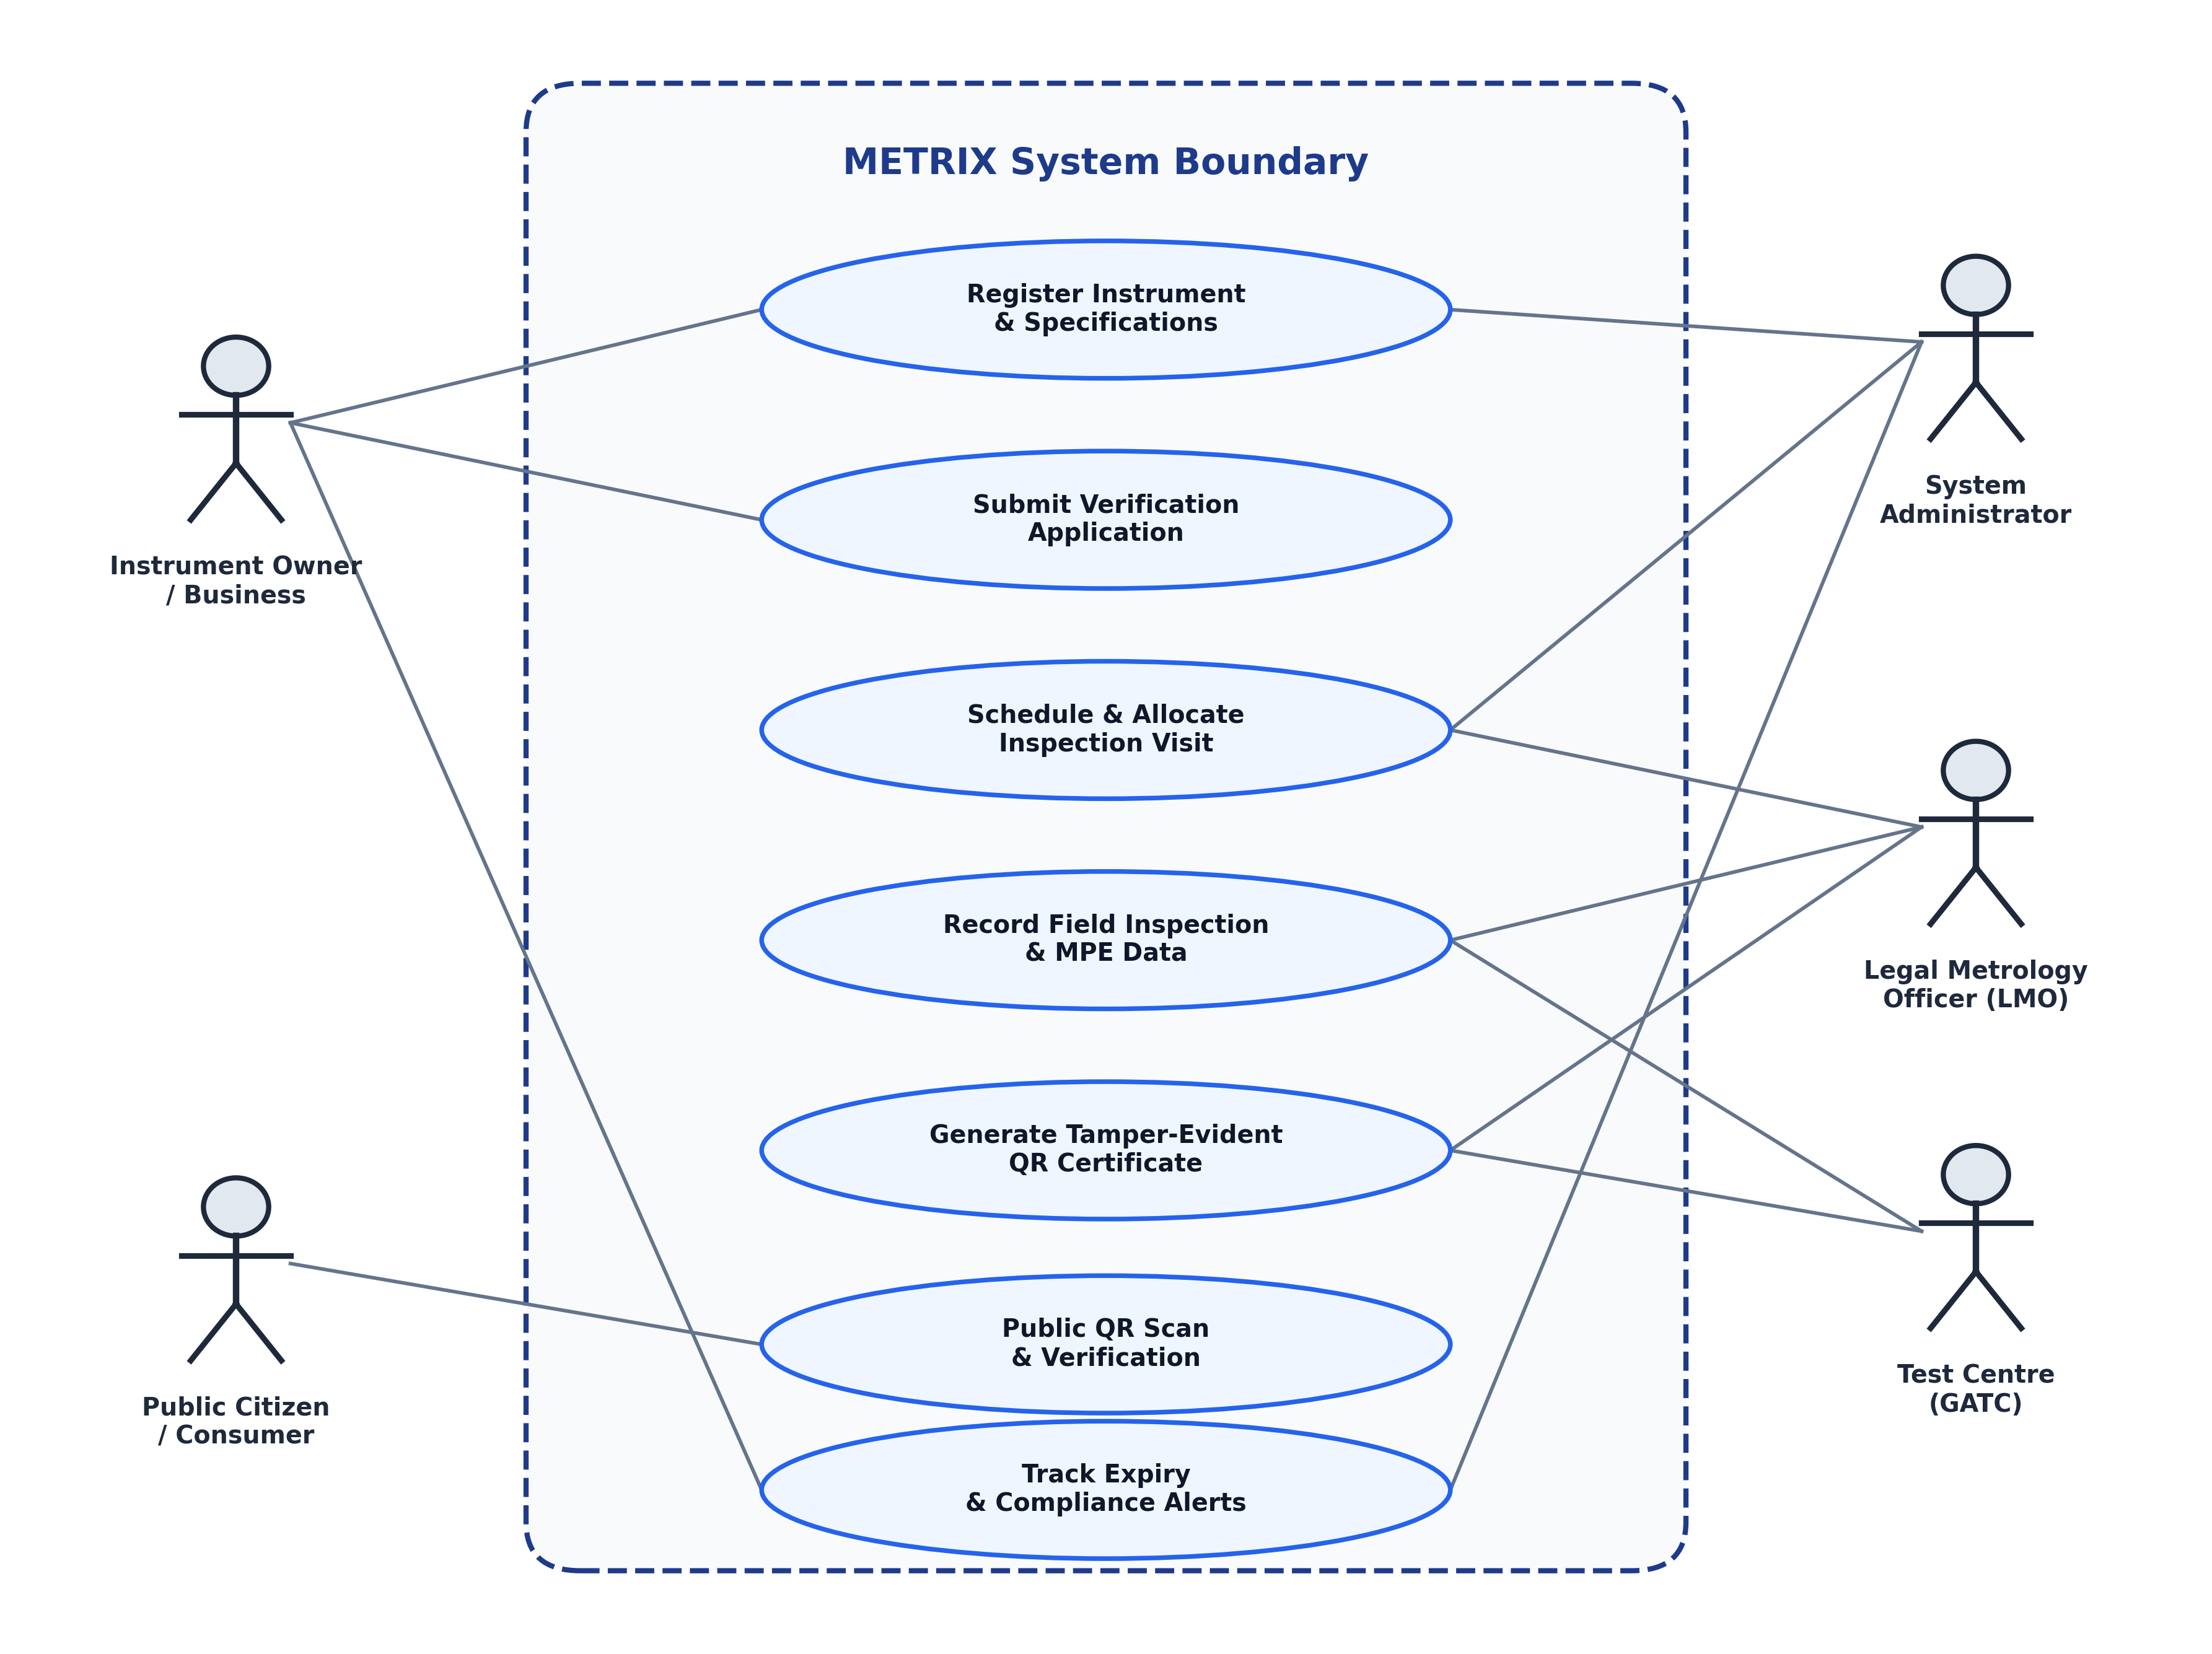
\includegraphics[width=0.95\textwidth]{use_case_diagram.png}
\caption{UML Use Case Diagram of the METRIX System}
\label{fig:use_case_diagram}
\end{figure}

\section{System Interfaces}
\begin{itemize}
    \item \textbf{Software Interfaces:} Next.js (TypeScript, Tailwind CSS) communicating via RESTful JSON APIs with a FastAPI (Python 3.10+) backend, persisting data in PostgreSQL 14+ via SQLAlchemy 2.x ORM. Certificates are generated via ReportLab and Python \texttt{qrcode}.
    \item \textbf{Hardware Interfaces:} Standard desktop, tablet, and mobile browsers, utilizing integrated device cameras for optical QR code scanning.
    \item \textbf{Communication Protocols:} Secure HTTPS/TLS 1.3 transport using JSON data payloads and HTTP \texttt{Authorization: Bearer <JWT>} headers.
\end{itemize}

\section{System Requirements and Constraints}
\begin{itemize}
    \item \textbf{Minimum Hardware:} Dual-Core CPU, 4 GB RAM, 10 GB SSD storage.
    \item \textbf{Software Stack:} Linux / Windows OS, Python 3.10+, Node.js 18+, PostgreSQL 14+.
    \item \textbf{Security \& Integrity:} Salted bcrypt password hashing, stateless JWT session tokens, and SHA-256 cryptographic digest embedded into certificates for tamper detection.
    \item \textbf{Architectural Constraints:} Software-only modular monolith; explicitly excludes Docker, Kubernetes, Redis, message queues, and external cloud dependencies.
\end{itemize}
